\documentclass[12pt]{article}

%Paquetes a utilizarse
\usepackage[width=7in, height=9.5in, top=0.75in, papersize={8.5in,11in}]{geometry}
\usepackage[spanish]{babel} 
\decimalpoint
\usepackage[utf8]{inputenc}
\usepackage{bbding}
\usepackage[colorlinks = true, linkcolor = blue, urlcolor = BlueViolet, citecolor = OliveGreen]{hyperref}
\usepackage{graphicx}
\usepackage{amssymb,amsthm,amsmath}
\usepackage{enumerate}
\usepackage{array,multicol,multirow}
\usepackage{xcolor}
\usepackage{fancybox,tcolorbox}
\usepackage{caption,subcaption,float,tabularx}
\usepackage{enumitem}

\theoremstyle{definition}
\newtheorem{corolario}{Corolario}
\newtheorem{lema}[corolario]{Lema}
\newtheorem{proposicion}[corolario]{Proposición}
\newtheorem{teorema}[corolario]{Teorema}
\newtheorem{propiedad}[corolario]{Propiedad}
\newtheorem*{observacion}{Observación}
\newtheorem{definicion}{Definición}
\newtheorem*{demostracion}{Demostración}
\newtheorem{ejemplo}{Ejemplo}
\newtheorem{problema}{Problema}
\newtheorem*{solucion}{Solución}
\newtheorem{ejercicio}{\PencilRightDown \  Ejercicio}
\newtheorem{step}{Paso}
\newtheorem{credito}{Crédito}

\usepackage{tikz}
\usetikzlibrary{arrows.meta,babel,calc,positioning}

\renewcommand{\arraystretch}{1.5}
\providecommand{\abs}[1]{\lvert#1\rvert}
\providecommand{\norm}[1]{\lVert#1\rVert}

\renewcommand{\tabularxcolumn}[1]{m{#1}}
\newcommand{\Evaluacion}[4]{
\setcounter{ejercicio}{0}
\noindent\begin{tabular}{lcr}
	\includegraphics[height=3cm]{Logos/logo-UES.png}\hspace{2.5em}
	&
	\includegraphics[height=2.75cm]{Logos/logo-PJT.png}
	& 
	\hspace{2.5em}\includegraphics[height=2.75cm]{Logos/logo-MINEDUCYT.png}
\end{tabular}

\hfill

\begin{center}
    
    UNIVERSIDAD DE EL SALVADOR
    \\PROGRAMA JÓVENES TALENTO
    \\FDTC 2022
    \\#2
    \\Nivel Olímpico C de Matemáticas

\end{center}

\begin{center}
    #1
\end{center}

%\textbf{Nombre}: \enspace\hrulefill

#3

\input{#4}
\newpage
}

\newtheorem{obs}{Observación}

%\usepackage[margin=2.5cm]{geometry}
%\usepackage{wasysym}
%\usepackage{stmaryrd,textcomp}
%\usepackage{pgf,tikz}
%\usetikzlibrary{arrows}

\parskip = 2mm   %%%% genera un espacio de X mm entre lo párrafos
\parindent = 3mm
\usepackage{multicol}
\usepackage{iwona}

\newcommand{\tema}{Combinaciones}
\newcommand{\fecha}{Viernes, 2 de diciembre de 2022}
\newcommand{\sesion}{Sesión 3}

\begin{document}
%\thispagestyle{empty}
%\newpage
\thispagestyle{empty}

\begin{figure}[h] 
	\begin{minipage}[b]{0.26\textwidth}
		\begin{center}
			
\includegraphics[height=3cm]{Logos/UES.png}
			\par\end{center}
	\end{minipage} 
	\begin{minipage}[b]{0.46\textwidth}
		\begin{center}
			UNIVERSIDAD DE EL SALVADOR\\ [0.1cm]
			PROGRAMA JÓVENES TALENTO\\ [0.1cm]
	        FDTC 2022\\ [0.1cm]
                NIVEL 5\\ [0.1cm]
			COMBINATORIA 
			\par\end{center}
	\end{minipage} 
	\begin{minipage}[b]{0.05\textwidth}
		\begin{center}
			
\includegraphics[height=2cm]{Logos/LOGO PJT.png}
			\par\end{center}
	\end{minipage}
\end{figure}

\begin{center}
    \begin{tabular}{p{4.5cm} p{7cm} p{4.5cm}}
        \tema & \centering\fecha & \hfill\sesion
    \end{tabular}
\end{center}

\section{Factorial de un número}

\subsection{Definición}

\begin{definicion}
    Se llama \textbf{factorial} de un número $n \in \mathbb{Z}^+_0$, al producto de los $n$ factores consecutivos desde $1$ hasta $n$ y se denota por $n!$, es decir,
\end{definicion}

\begin{center}
    $n! = (1)\cdot (2)\cdot (3)\cdots (n-1)\cdot (n)$.
\end{center}

En consecuencia, $1!=1$ y $n!=n(n-1)!$, por convención, definimos $0!=1$.

\begin{ejemplo}
    Algunas formas de trabajar con factoriales:
    \renewcommand{\labelenumi}{\alph{enumi})}
    \begin{enumerate}
        \item $4! = 4 \cdot (3) \cdot (2) \cdot (1) = 24$.
        \item $\frac{8!}{5!}= \frac{8 \cdot (7)\cdot (6)\cdot  (5!)}{5!}= 8 \cdot (7)\cdot  (6) = 336$.
        \item $\frac{12 \cdot(11)\cdot (10)}{3\cdot (2)\cdot (1)}= \frac{12\cdot (11) \cdot(10)\cdot (9!)}{3\cdot (2)\cdot (1)\cdot (9!)}= \frac{12!}{3! (9!)}$.
    \end{enumerate}
\end{ejemplo}

\subsection{Ejercicios}

\begin{ejercicio}
    Determinar el valor de x sabiendo que:
    \renewcommand{\labelenumi}{\alph{enumi})}
    \begin{enumerate}
        \item $x! = 110 (x-2)!$
        \item $12 (x!) + 5 (x+1)!=(x+2)!$
    \end{enumerate}
\end{ejercicio}

\begin{ejercicio}
    ¿De cuántas formas diferentes se pueden ordenar las letras de la palabra ''IMPUREZA''?
\end{ejercicio}

\begin{ejercicio}
    ¿De cuántas formas se pueden colocar 5 libros diferentes en fila en un mostrador?
\end{ejercicio}

\section{Combinaciones}

\subsection{Definición (Modelo de conjuntos)}

\begin{definicion}
    Una \textbf{combinación}  es cualquier selección de $r$ elementos de un conjunto de $n$ elementos distintos, de modo que el orden de selección no importa. Naturalmente, las combinaciones tienen una gran importancia en la combinatoria, y es de especial interés calcular, o contar, el número total de combinaciones que pueden resultar de una determinada selección de elementos de un conjunto.
\end{definicion}

\begin{definicion}
    Para cumplir este fin, se introduce la idea de \textbf{número combinatorio}, que se define como el número de formas en las que se pueden seleccionar $r$ elementos de un conjunto de $n$ elementos sin importar el orden, es decir, el número de combinaciones de $r$ elementos en $n$ elementos. En términos de conjuntos, también se puede entender como la cantidad de subconjuntos de $r$ elementos que se pueden formar a partir de un conjunto de $n$ elementos.
\end{definicion}

Los números combinatorios se denotan por:

\begin{center}
    $_{n}C_{r}$, $C^{r}_{n}$, $C_{n,r}$, $C(n,r)$, o $\binom{n}{r}$.
\end{center}

Ahora, antes de plantear la fórmula general de una combinación, veamos el siguiente ejemplo:

\begin{ejemplo}
    Se dispone de un grupo de 3 mujeres y 4 hombres.
    \renewcommand{\labelenumi}{\alph{enumi})}
    \begin{enumerate}
        \item ¿De cuántas maneras se puede seleccionar una pareja de dos personas del mismo sexo?
        \item ¿De cuántas maneras se puede seleccionar un grupo de 4 personas compuesto por 2 mujeres y 2 hombres?
    \end{enumerate}
\end{ejemplo}

\begin{solucion}
    Calculemos primero las parejas de mujeres. Nombrémos a las 3 mujeres $x, y, z$. Inicialmente, por el principio de la multiplicación, podríamos pensar que hay un total de $3 (2) = 6$ parejas de mujeres. Sin embargo, al evaluar las posibilidades, estaríamos contando las parejas $xy, yx, xz, zx, yz, zy$, como si el orden en el que se eligieran las integrantes de la pereja fuera importante, es decir, como si la pareja $xy$ fuera distinta a la pareja $yx$. Entonces, de qué manera podemos eliminar las parejas repetidas. La solución pasa por dividir el total de posibilidades entre el número de configuraciones internas que pueda tener cada pareja, es decir, $2!$. Entonces, en total, habrían $\frac{3 (2)}{2!} = 3$ posibles parejas de mujeres. 
    
    Análogamente, la misma situación sucede con las parejas de hombres, donde el número total de parejas, evitando las repeticiones, sería $\frac{4 (3)}{2!}=6$. En total, por el principio de la suma, se tienen $3+6=9$ posibilidades.
    
    Para el literal b, únicamente, por el principio de la multiplicación, hay que calcular el producto de las posibles parejas de mujeres con las posibles parejas de hombres, es decir, $6 (3) = 18$. En total hay $18$ posibles grupos de 4 personas formados por una pareja de hombres y otra de mujeres.
\end{solucion}

Este problema ha presentado una situación en la que, a partir de un conjunto de elementos disponibles, se deben seleccionar algunos de ellos, es decir, tenemos un problema de combinaciones. Entonces, expresadas como números combinatorios, las soluciones del problema vendrían dadas por:

\renewcommand{\labelenumi}{\alph{enumi})}
\begin{enumerate}
    \item $C^{2}_{3}+C^{2}_{4} = \binom{3}{2}+\binom{4}{2} = 9$
    \item $ C^{2}_{3} \cdot C^{2}_{4} = \binom{3}{2} \cdot \binom{4}{2} = 18$
\end{enumerate}

\subsection{Fórmula general}

A partir del ejemplo anterior, podemos deducir que el total de combinaciones resultante de seleccionar $r$ elementos de un conjunto de $n$ es igual a:

\begin{center}
    $ C^{r}_{n}= \binom{n}{r} = \frac{n (n-1)(n-2)...(n-r+1)}{r!}$
\end{center}

Pero,  $n (n-1)(n-2)...(n-r+1)=\frac{n!}{(n-r)!}$, por lo que obtenemos:

\begin{center}
    $ C^{r}_{n}= \frac{n!}{(n-r)! \ r!}$
\end{center}

\subsection{Problemas}

\begin{problema}
    Se dispone de los números 1, 2, 3, 4, 5 y 6 para llenar tres casillas en blanco, escribiendo un número en cada casilla y tal que los tres números utilizados sean distintos entre sí.
    
    \begin{center}
        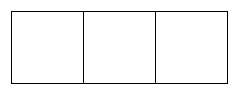
\includegraphics[scale=0.4]{Imagenes/IMG1/ejem.png}
    \end{center}
    
    \renewcommand{\labelenumi}{\alph{enumi})}
    \begin{enumerate}
        \item ¿De cuántas formas se puede hacer?
        \item Si al llenar las casillas, los números seleccionados se ubican en orden creciente, ¿de cuántas maneras se puede hacer?
    \end{enumerate}
\end{problema}

\begin{solucion}
    Para el literal a, el problema se reduce a seleccionar ordenadamente 3 de los 6 números disponibles. La solución se reduce a:

    \begin{center}
        $6 (5) (4)= 120$.
    \end{center}

    Para el literal b, hay que notar que, para cada combinación de 3 números, existe solo un orden correcto en el que los números se dispongan de manera creciente, es decir, una vez que se escoja la combinación la forma de úbicarlos es única. Por lo tanto, la solución es 
    
    \begin{center}
        $C^{3}_{6}=\frac{6!}{(6-3)! \ 3!}= \frac{6 (5) (4)}{3!}=20$.
    \end{center}
\end{solucion}

\begin{problema}
    Una panadería hace sandwiches según la elección del cliente, ofreciendo 3 tipos diferentes de panes y 10 tipos diferentes de rellenos. Si  el  cliente  puede  escoger  un  tipo  de  pan  y  1,  2  o  3  rellenos  diferentes, determine el número de maneras de componer el Sandwich.
\end{problema}

\begin{solucion}
    Como tenemos tres tipos de panes para escoger uno, tenemos  3  posibilidades  de  hacer  la  elección.  Si  quisiéramos  escoger exactamente  un  relleno  tenemos $\binom{10}{1}=10$  posibilidades. Si queremos  escoger  dos  tipos  de  relleno  tenemos $\binom{10}{2}=45$ posibilidades.   Por  otro  lado,  si  queremos  escoger  tres  tipos  de  relleno  setienen $\binom{10}{3}=120$ posibilidades. Entonces, pro el principio de la multiplicación, en total hay $3(10+45+120)=525$ posibilidades.
\end{solucion}

\begin{problema}
    ¿Cuántos diferentes licuados mezclando dos frutas pueden hacerse si se dispone de fresas, uvas, bananos, coco, piña, zapote y melón? ¿Cuántos con tres frutas?
\end{problema}

\begin{problema}
    Se tiene el conjunto $\{a, b, c, d, e\}$. ¿Cuántos y cuáles de sus subconjuntos tienen una letra, dos letras, tres letras, cuatro letras, cinco letras y ninguna letra?
\end{problema}

\begin{problema}
    De un grupo de seis hombres y cuatro mujeres se desea formar una comisión de tres personas. Cuántas comisiones distintas se pueden formar si:

    \renewcommand{\labelenumi}{\alph{enumi})}
    \begin{enumerate}
        \item no hay más restricciones?
        \item debe haber un hombre y dos mujeres?
        \item debe haber al menos un hombre?
    \end{enumerate}
\end{problema}

\begin{problema}
    Si se dispone de cinco puntos en el plano, de los cuales no hay tres alineados, ¿cuántos segmentos de recta que unan dos de dichos puntos se pueden trazar?
\end{problema}

\begin{problema}
    ¿Cuántos triángulos se pueden formar utilizando los vértices de un polígono regular de 10 lados?
\end{problema}

\begin{problema}
    De un grupo de 24 personas, se quieren elegir a 5 representantes de la siguiente forma: Manuel y Luis deben estar en el grupo elegido. Hay 8 mujeres en total, pero como máximo deben figurar 2 en el grupo. ¿De cuántas maneras distintas se puede hacer la elección?
\end{problema}

\begin{problema}
    Un grupo de 15 alumnos quiere dividirse en 3 equipos de 5 alumnos cada uno. ¿De cuántas maneras puede hacerse la distribución si todos hablarán del valor de la honestidad?
\end{problema}

\begin{problema}
    Un grupo de 15 alumnos quiere dividirse en 3 equipos de 5 alumnos cada uno. ¿De cuántas maneras puede hacerse la distribución si un grupo debe hablar del valor de la honestidad, otro de la solidaridad y el último de la cooperación?
\end{problema}

\begin{problema}
    En el entrenamiento de la Olimpiada Matemática, $n$ estudiantes se saludan entre sí (una sola vez). ¿Cuántos saludos ocurren? 
\end{problema}

\begin{problema}
    En una fila hay 5 pelotas rojas y 9 pelotas azules, y se quiere forma una fila con todas ellas. ¿De cuántas maneras se puede formar la fila? ¿De cuántas maneras si no pueden haber dos rojas consecutivas?
\end{problema}

\begin{problema}
    Encuentre el número de formas de poner 3 torres en un tablero de ajedrez de $5 \times 5$, sin que cualesquiera dos de ellas se ataquen. ¿Y si fueran $n$ torres en un tablero de $n \times n$?
\end{problema}

\newpage

\subsection{Modelo de cadenas binarias}

Hasta el momento se ha dicho que $C^{k}_{n}$ puede interpretarse como la cantidad de subconjuntos de $k$ elementos de un conjunto de cardinalidad $n$, es decir, la cantidad de formas de escoger $k$ objetos entre $n$ objetos diferentes. Ahora bien, esta interpretación de un número combinatorio puede asociarse a otro problema:¿Cuántas cadenas de unos y ceros se pueden formar con $k$ unos y $n-k$ ceros?

Podemos interpretar esto como tener a disposición $n$ espacios vacíos en los que se debe colocar o bien un 1 o bien un 0.

\begin{center}
    $\underbrace{1\ 0\ 0\ 1\ 0\ 1...0\ 1\ 1\ 0}_{n}$
\end{center}

Además se tiene prefijada la cantidad de unos y ceros que deben colocarse en esos $n$ espacios, en total son exactemente $k$ unos y, por ende, los restantes $n-k$ deben ser ceros.  Entonces basta conocer de cuántas formas puedo colocar los unos y luego las posiciones de los ceros quedan determinadas. Es así como se tiene que
la cantidad de cadenas de longitud $n$ de $k$ unos y $n-k$ ceros está dada por $C^{k}_{n}$.

\begin{ejemplo}
    Pruebe usando cadenas de ceros o unos que:
    \begin{center}
        $C^{k}_{n}=C^{k-2}_{n-2}+2C^{k-1}_{n-2}+C^{k}_{n-2}$
    \end{center}
\end{ejemplo}

\begin{solucion}
    Asumamos que $k$ es la cantidad de unos, así que $C^{k}_{n}$ cuenta de golpe la cantidad de tales cadenas de longitud $n$. Bajo la misma idea, ¿qué podemos decir de los 3 términos de la derecha?

    Para $C^{k-2}_{n-2}$ son las cadenas de longitud $n-2$ pero con $k-2$ unos. Para hacerlas de longitud $n$ con $k$ unos. se agrega al final de estas 11, al hacerlo obtenemos el total de cadenas delongitud $n$ conkunos pero que terminan en 11.

    Para $2C^{k-1}_{n-2}$ son las cadenas de longitud $n-1$ pero con $k-1$ unos. Para hacerla de longitud $n$ con $k$ unos, se agrega al final de estas 01 o 10.  Demanera que hay dos formas para las cadenas calculadas, por ello el coeficiente 2.

    Para $C^{k}_{n-2}$ son las cadenas de longitud $n-2$ con $k$ unos. Para hacerla de longitud $n$, debemos llenar dos espacios con ceros, es decir, 00, ya que los unos están completos.

    Como cada caso es excluyente del resto, por el principio de la suma tenemos el resultado:

    \begin{center}
        $C^{k}_{n}=C^{k-2}_{n-2}+2C^{k-1}_{n-2}+C^{k}_{n-2}$
    \end{center}
\end{solucion}

\begin{problema}
    ¿Cuántas cadenas de longitud 7 se pueden formar con 4 ceros y 3 unos?
\end{problema}

\begin{problema}
    ¿Cuántas cadenas de longitud $n$ se pueden formar con $k$ unos y $n-k$ ceros?
\end{problema}

\begin{problema}
    ¿Cuántas cadenas de longitud 6 contienen como máximo 3 unos?
\end{problema}

\newpage

\subsection{Modelo de caminos}

Suponga  la  siguiente  situación,  una  persona se encuentra de paseo en una ciudad y está interesada en ir de la esquina A hasta la esquina B por la ruta más corta posible, tal como lo muestra la siguiente figura:

\begin{center}
    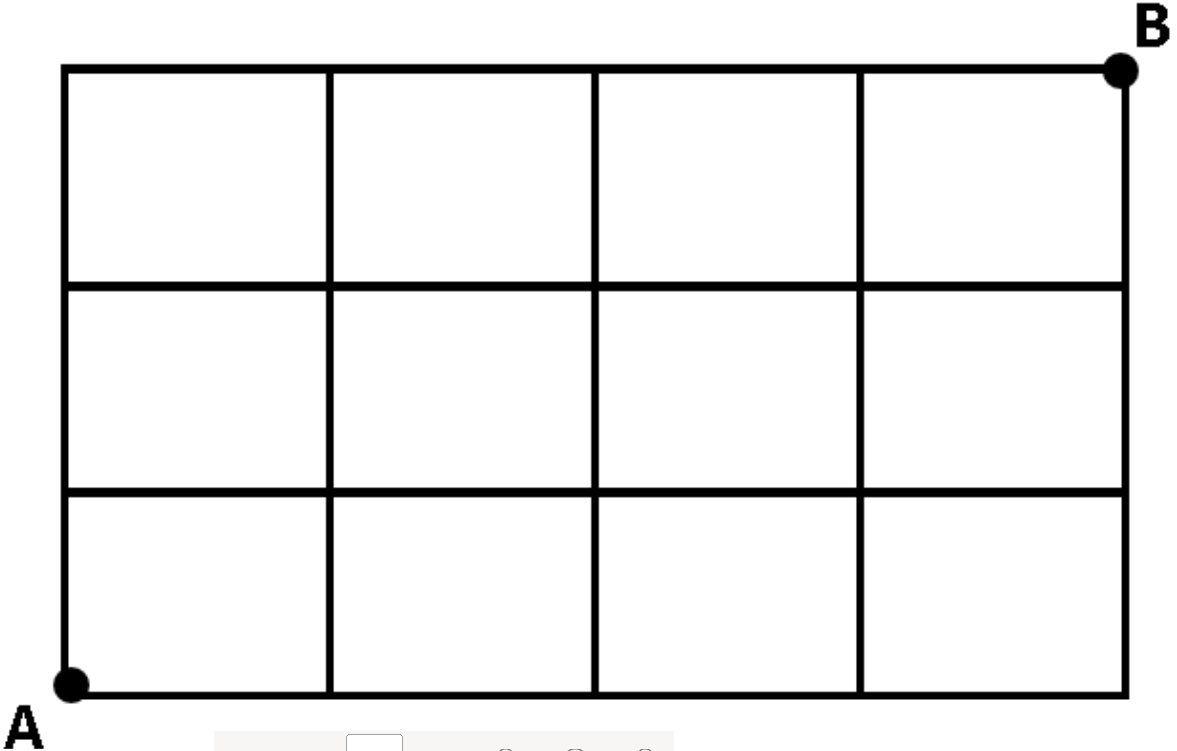
\includegraphics[scale=0.4]{Imagenes/IMG3/Caminos1.png}
\end{center}

¿De cuántas formas podemos realizar dicho recorrido?

En primer lugar, hay que notar que los caminos de longitud mínima deben estar formados por 4 movimientos a la derecha y 3 hacia arriba. Así que cada camino se puede asociar a un arreglo de 4 símbolos $\rightarrow$ y y 3 símbolos $\leftarrow$, lo cual puede hacerse de $\binom{7}{4}$ maneras. 

En general, dada una cuadrícula de dimensión $k \times (n-k)$, como la siguiente:

\begin{center}
    \includegraphics[scale=0.8]{Imagenes/IMG3/Caminos2.png}
\end{center}

La cantidad de caminos de longitud mínima que llevan del punto A al punto B viene dada por el número combinatorio 

\begin{center}
    $C^{k}_{n}=C^{n-k}_{n}$
\end{center}

\begin{problema}
    En cada una de las cuadrículas, expresar usando números combinatorios (no es necesario calcularlos) ¿cuántos caminos de longitud mínima comienzan en el punto A y terminan en el punto B?

    \begin{center}
        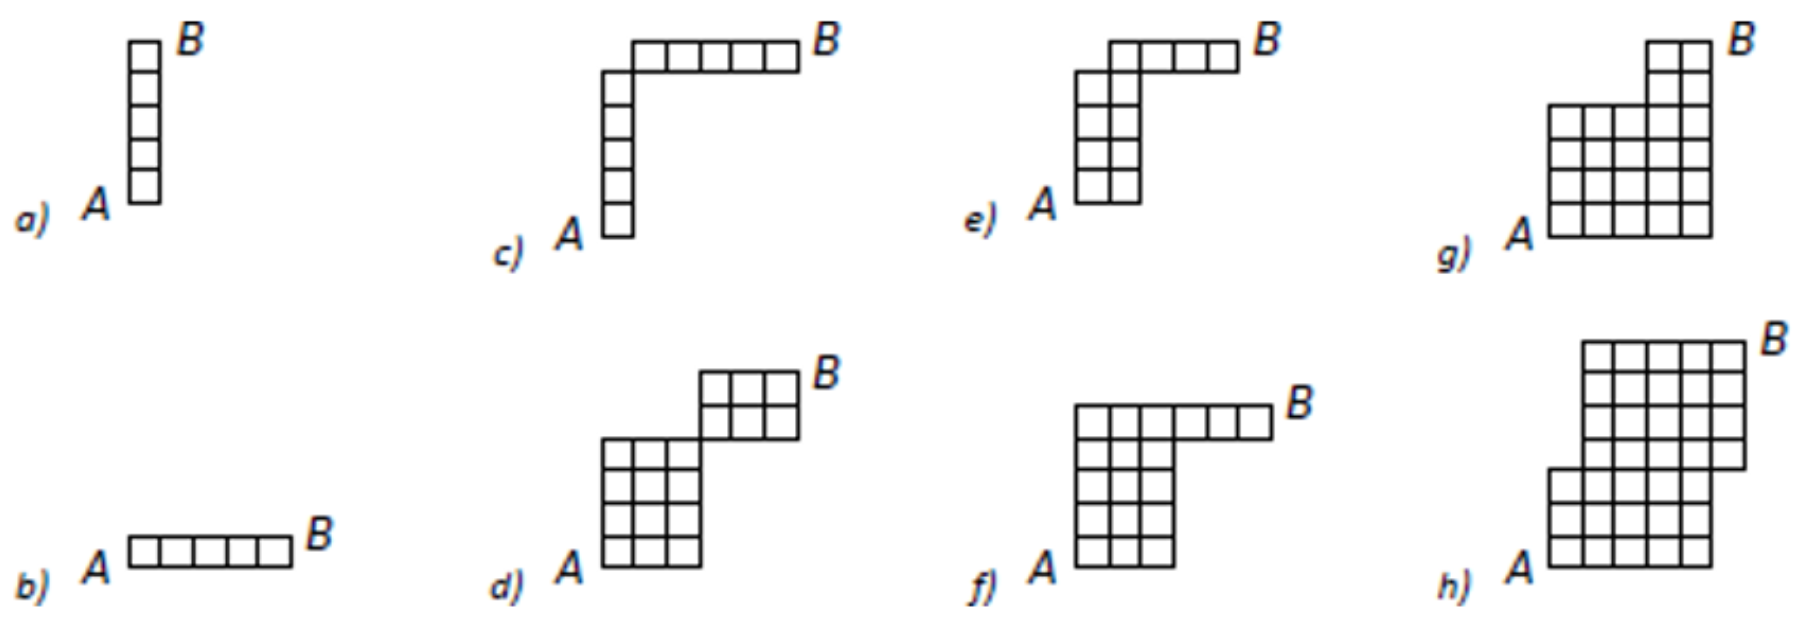
\includegraphics[scale=0.5]{Imagenes/IMG3/Caminos3.png}
    \end{center}
    
\end{problema}
    
\begin{problema}
    Considerar la cuadrícula y que solo se permiten movimientos hacia la derecha o hacia arriba. Responder cuántos caminos de longitud mínima llevan:

    \begin{center}
        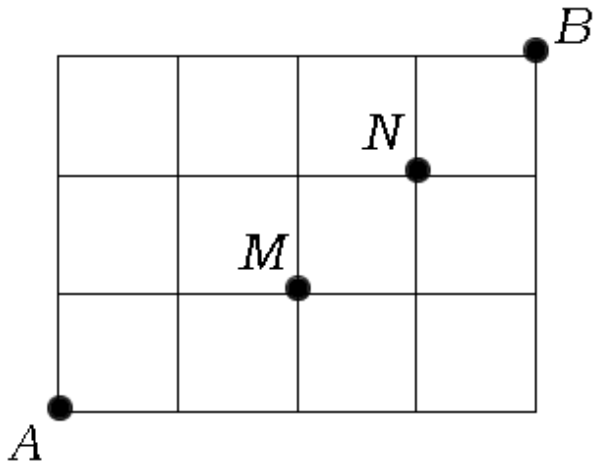
\includegraphics[scale=0.6]{Imagenes/IMG3/Caminos4.png}
    \end{center}

    \begin{itemize}
        \item De A a M.
        \item De M a B.
        \item De A a B pasando por M.
        \item De A a B pasando por N.
        \item De A a B pasando por M y N.
        \item De A a B pasando por M o N.
        \item De A a B y no pasan ni por M ni por N.
    \end{itemize}
    
\end{problema}



\end{document}